\documentclass[12pt]{article}
\usepackage{hyperref}
\usepackage{authblk}
\usepackage{graphicx}
\usepackage{amsmath}
\usepackage{amssymb}
\usepackage{enumitem}
\usepackage{amsfonts}
\usepackage{array}
\usepackage{xcolor}
\usepackage{tikz}
\usepackage{pifont}
\usepackage{fontawesome5}
\usepackage{tikz-3dplot}
\usepackage{forest}
\usepackage{cancel}
\usepackage{ulem}
\usepackage{subcaption}
\usepackage{booktabs}
\usepackage{placeins}
\usepackage[margin=1in]{geometry}

\title{Forecasting Grocery Store Product Sales}
\author{Austin Lackey}
\author{Tomy Sabalo Farias}
\author{Sam Herold}
\affil{DSCI 478, Colorado State University}

\begin{document}

\maketitle

\begin{abstract}
This paper presents a methodology for forecasting grocery store sales across many stores and product subsets.
The data used in this project is from Favorita Grocery Stores in Ecuador from 2013 to 2017 and is provided by Kaggle.
A link to the data can be found in the references section at the end of this paper.
Our methodology is split into three main sections: data preprocessing, model engineering, and model evaluation.
In this project, we use a variety of models including linear and polynomial regression and gradient boosting.
\end{abstract}

\section{Introduction and Background}
The 'Store Sales' time series forecasting dataset contains sales data from Favorita Grocery Stores in Ecuador from 2013 to 2017.
Sales data is broken down by store and product category for each day (pair-wise combinations $stores \times products$).
The goal of this project is to forecast sales for each store and product category for any given day in the future.
Below is a brief description of the variables that were provided in the raw dataset.
% insert table here, header: variable, unique counts, description
\begin{table}[h]
\centering
\begin{tabular}{|c|c|c|c|}
\hline
\textbf{Variable} & \textbf{Type} & \textbf{Unique Counts} & \textbf{Description} \\ \hline
date & datetime64 & 1684 & Date-stamp of the sales data \\ \hline
store\_nbr & int64 & 54 & Store number \\ \hline
family & categorical & 33 & Product family (Grocery, Beverages, Deli, etc.) \\ \hline
city & categorical & 22 & City of the store \\ \hline
state & categorical & 16 & State of the store \\ \hline
type & categorical & 5 & Type of store (A, B, C, D, E) \\ \hline
cluster & int64 & 17 & Cluster of the store (Similar stores grouped together) \\ \hline
\end{tabular}
\caption{Variable Descriptions}
\end{table}
\\
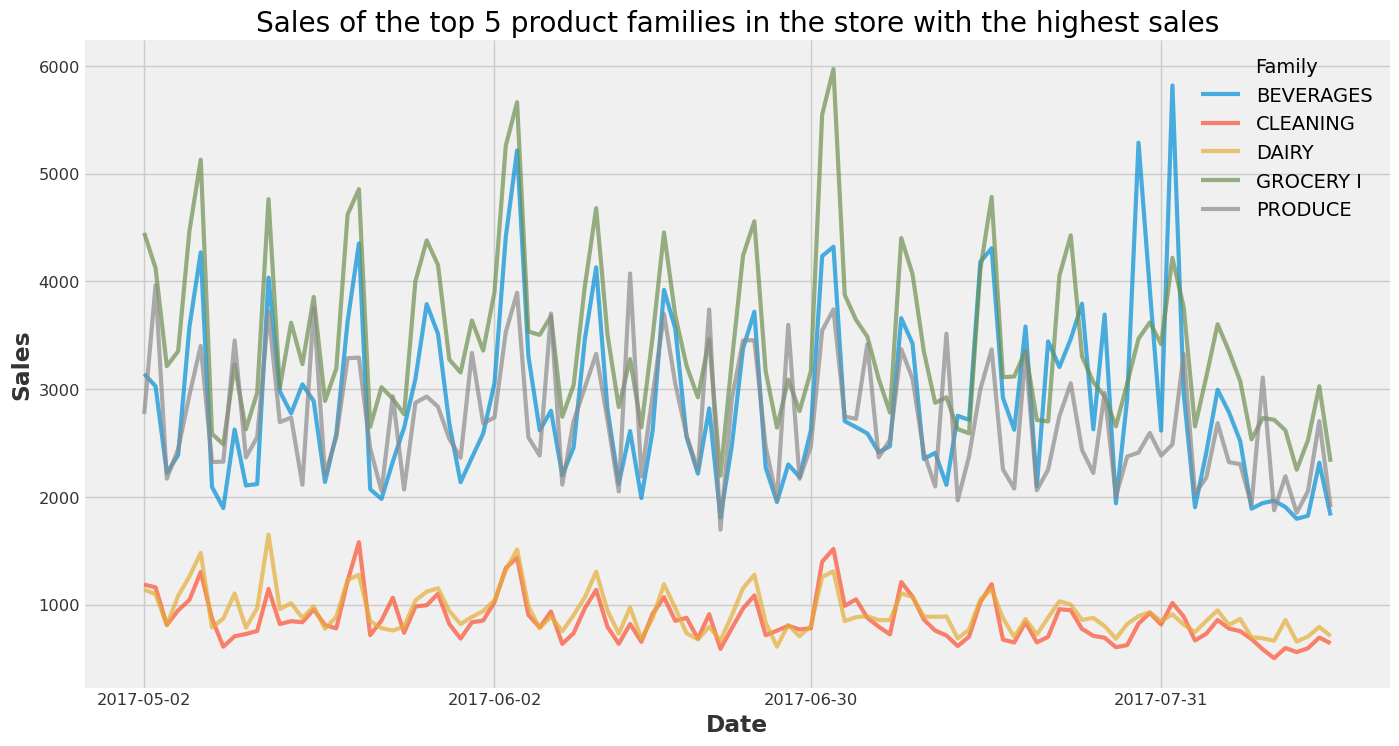
\includegraphics[width=\textwidth]{figures/Top 5 Products.png}
Fix plot and expand on it later...
% table to represent an example of pair-wise combinations
\begin{table}[h]
\centering
\begin{tabular}{|c|c|c|}
\hline
\textbf{Date} & \textbf{Store Number} & \textbf{Product Family} \\ \hline
2013-01-01 & 1 & Grocery \\ \hline
2013-01-01 & 1 & Beverages \\ \hline
2013-01-01 & 1 & Deli \\ \hline
\dots & \dots & \dots \\ \hline
2013-01-01 & 54 & Grocery \\ \hline
2013-01-01 & 54 & Beverages \\ \hline
2013-01-01 & 54 & Deli \\ \hline
\dots & \dots & \dots \\ \hline
2013-01-02 & 1 & Grocery \\ \hline
\dots & \dots & \dots \\ \hline
\end{tabular}
\caption{Example of Pair-Wise Combinations}
\end{table}
\section{Feature Engineering}
The biggest challenge in this project was to create a feature set that would allow us to forecast sales for each store and product category.
We found that the most important part in reducing $RMSE$ was to create a feature set that captured as much information regarding seasonality and trends as possible.
We created a feature set that included the following extra variables:
\begin{itemize}
    \item \textbf{Datetime Features:} We created features that captured what day of the week it was, the day of the month, the month, the quarter, the week of the year and the year.
    \item \textbf{Lag Features:} We implemented a 7-day lag feature to capture the previous week's sales that led up to the current day. This feature really helped the model fine-tune the forecast.
    \item \textbf{Store-Specific Features:} We joined the store data with the sales data to give the model more information about the store. 
\end{itemize}
Expand more here\dots
\section{Model Engineering}
Add intro here\dots \\
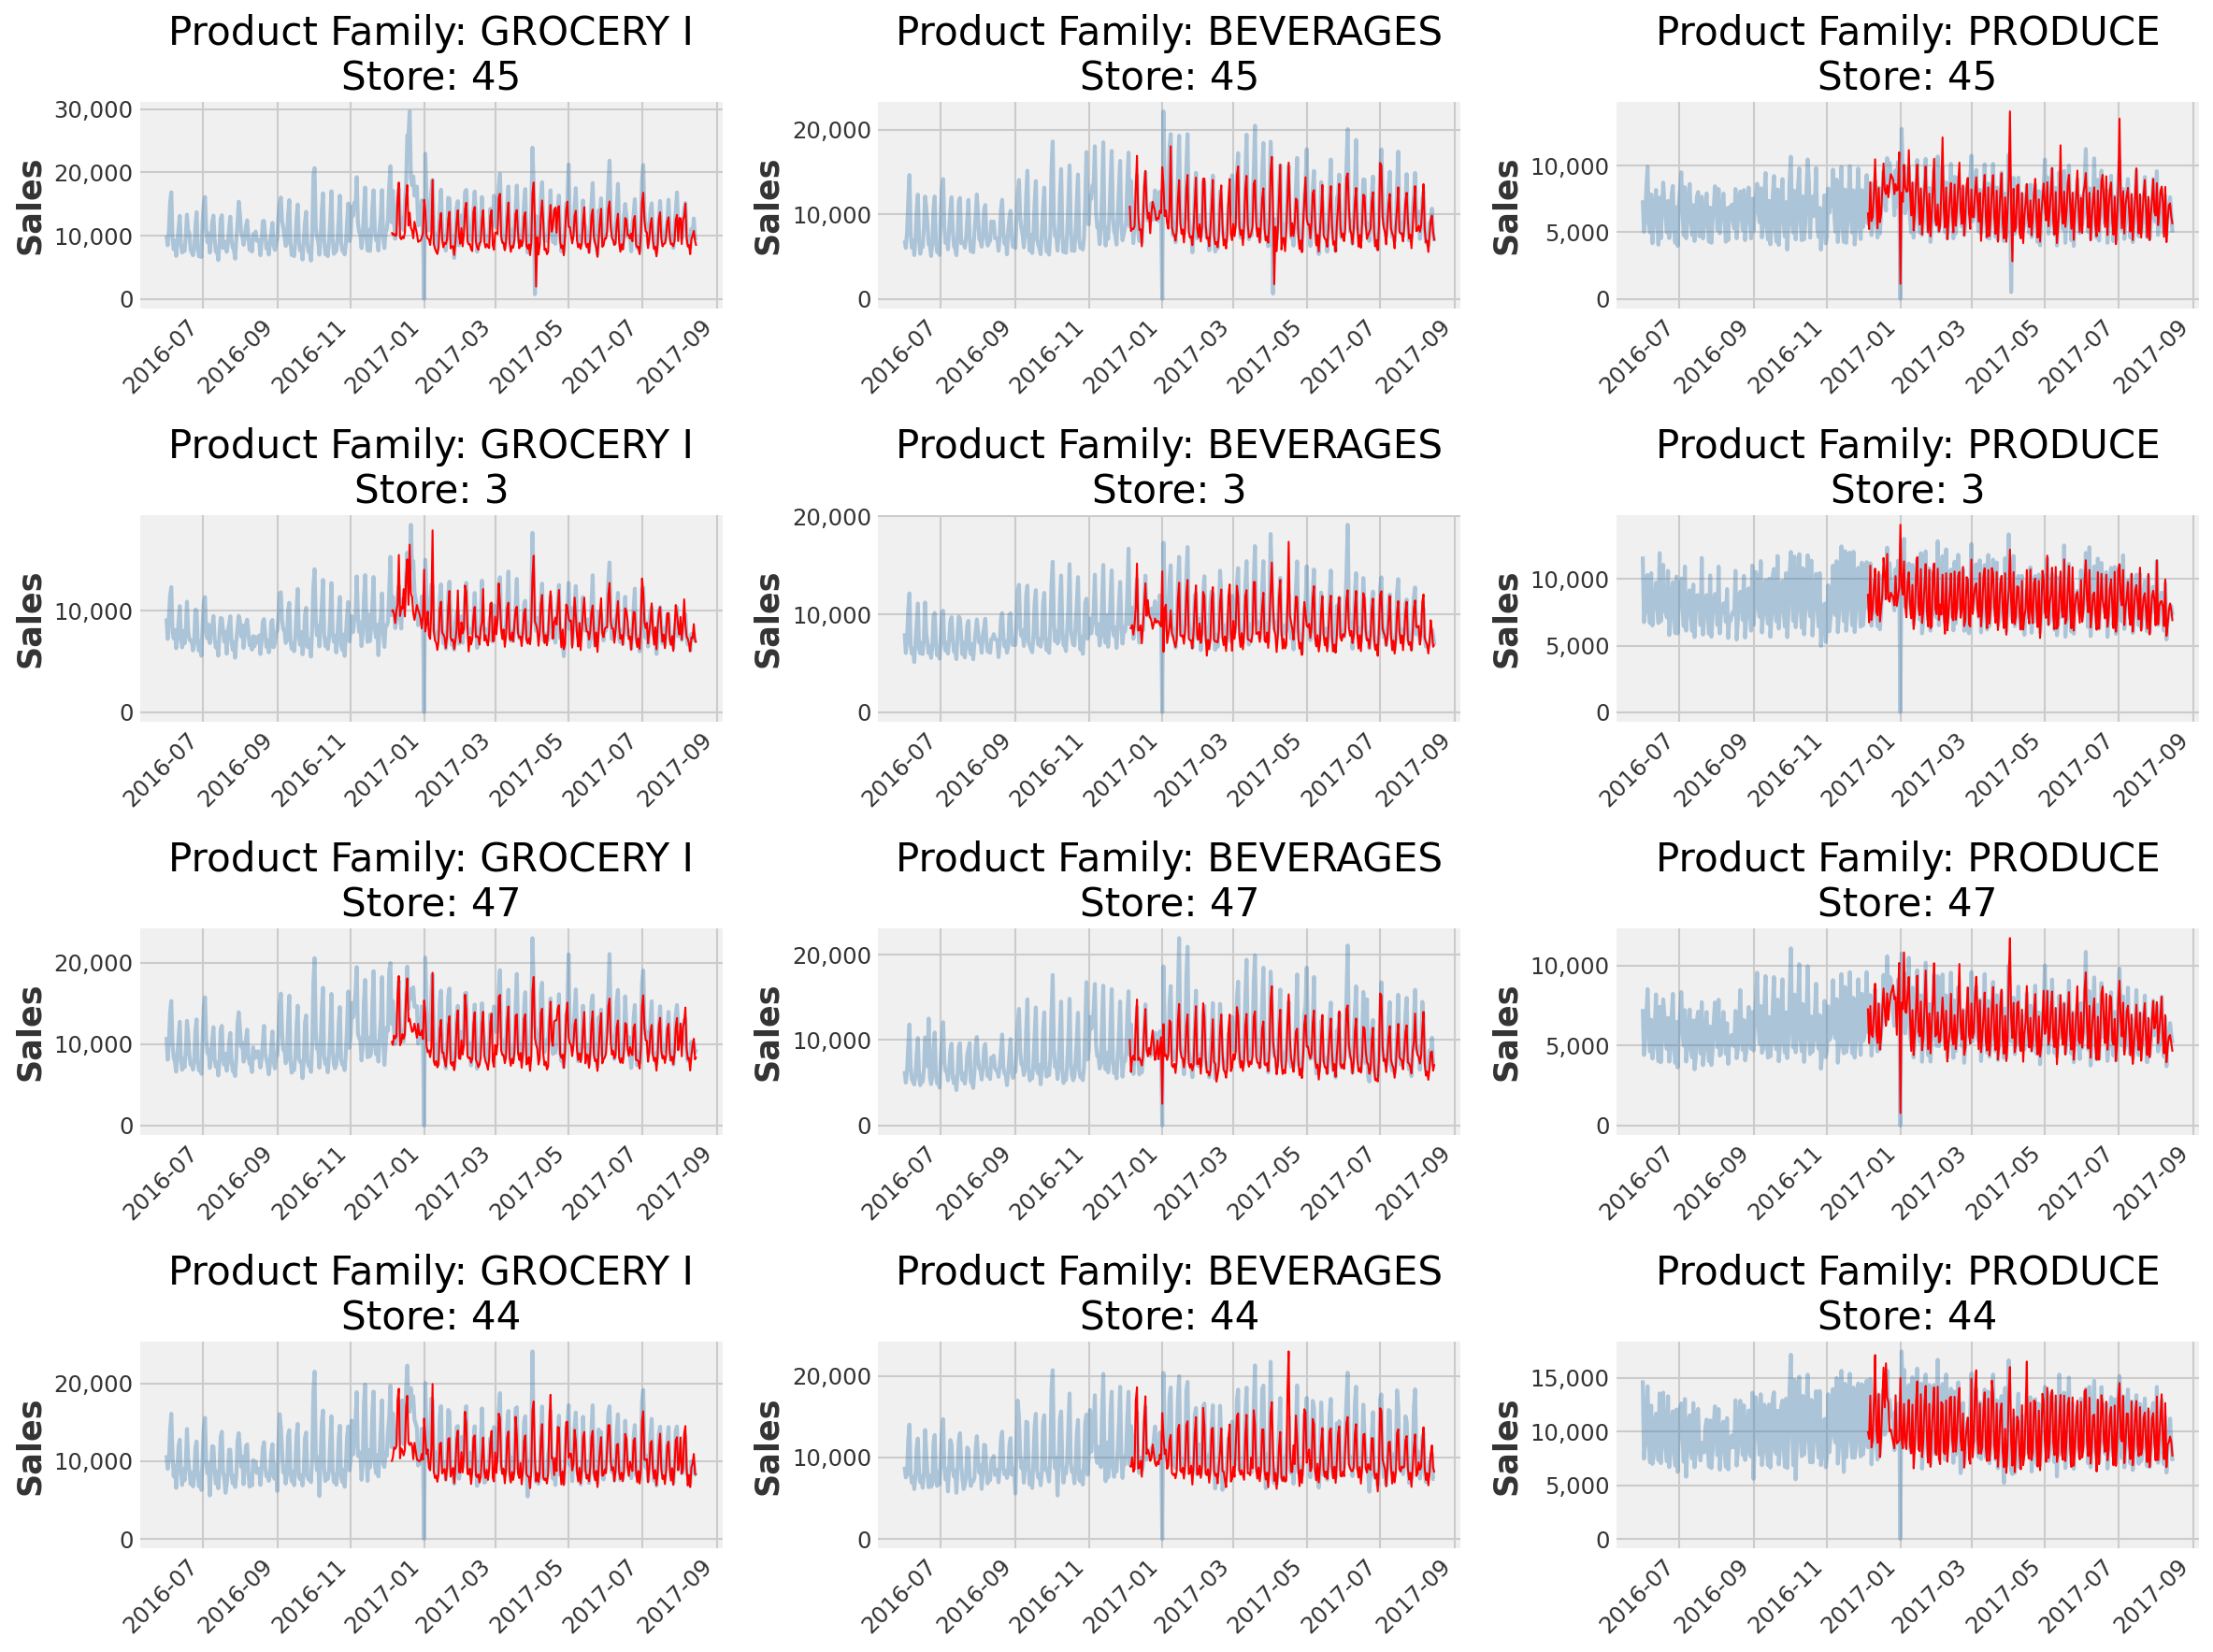
\includegraphics[width=\textwidth]{figures/XGBoost.png}
\end{document}